%% 
%% Copyright 2007-2020 Elsevier Ltd
%% 
%% This file is part of the 'Elsarticle Bundle'.
%% ---------------------------------------------
%% 
%% It may be distributed under the conditions of the LaTeX Project Public
%% License, either version 1.2 of this license or (at your option) any
%% later version.  The latest version of this license is in
%%    http://www.latex-project.org/lppl.txt
%% and version 1.2 or later is part of all distributions of LaTeX
%% version 1999/12/01 or later.
%% 
%% The list of all files belonging to the 'Elsarticle Bundle' is
%% given in the file `manifest.txt'.
%% 

%% Template article for Elsevier's document class `elsarticle'
%% with numbered style bibliographic references
%% SP 2008/03/01
%%
%% 
%%
%% $Id: elsarticle-template-num.tex 190 2020-11-23 11:12:32Z rishi $
%%
%%
\documentclass[preprint,12pt]{elsarticle}

% \usepackage[UTF8]{ctex}
% \usepackage{xeCJK} % 该命令与上一行等价

%% Use the option review to obtain double line spacing
%%\documentclass[authoryear,preprint,review,12pt]{elsarticle}

%% Use the options 1p,twocolumn; 3p; 3p,twocolumn; 5p; or 5p,twocolumn
%% for a journal layout:
%% \documentclass[final,1p,times]{elsarticle}
%% \documentclass[final,1p,times,twocolumn]{elsarticle}
%% \documentclass[final,3p,times]{elsarticle}
%% \documentclass[final,3p,times,twocolumn]{elsarticle}
%% \documentclass[final,5p,times]{elsarticle}
%% \documentclass[final,5p,times,twocolumn]{elsarticle}

%% For including figures, graphicx.sty has been loaded in
%% elsarticle.cls. If you prefer to use the old commands
%% please give \usepackage{epsfig}

%% The amssymb package provides various useful mathematical symbols
\usepackage{amssymb}
\usepackage{amsmath}
\usepackage{tabularx}
\usepackage{algpseudocode}
\usepackage[margin=3cm]{geometry}
\usepackage{algorithm2e}
\usepackage{textgreek}
\usepackage{color}
\usepackage{booktabs}
\usepackage{geometry}
\usepackage{makecell}
\usepackage{graphicx} 
\usepackage{caption} 
\usepackage{subcaption} 
\usepackage{fontspec}
\usepackage{xeCJK}

\geometry{left=1in, right=1in, top=1in, bottom=1in}

%% The amsthm package provides extended theorem environments
%% \usepackage{amsthm}

%% The lineno packages adds line numbers. Start line numbering with
%% \begin{linenumbers}, end it with \end{linenumbers}. Or switch it on
%% for the whole article with \linenumbers.
%% \usepackage{lineno}

\journal{Journal of Manufacturing Systems}

\begin{document}

\begin{frontmatter}

%% Title, authors and addresses

%% use the tnoteref command within \title for footnotes;
%% use the tnotetext command for theassociated footnote;
%% use the fnref command within \author or \address for footnotes;
%% use the fntext command for theassociated footnote;
%% use the corref command within \author for corresponding author footnotes;
%% use the cortext command for theassociated footnote;
%% use the ead command for the email address,
%% and the form \ead[url] for the home page:
%% \title{Title\tnoteref{label1}}
%% \tnotetext[label1]{}
%% \author{Name\corref{cor1}\fnref{label2}}
%% \ead{email address}
%% \ead[url]{home page}
%% \fntext[label2]{}
%% \cortext[cor1]{}
%% \affiliation{organization={},
%%             addressline={},
%%             city={},
%%             postcode={},
%%             state={},
%%             country={}}
%% \fntext[label3]{}

\title{An Edge Intelligence-based Model Deployment Method for CNC Systems}

%% use optional labels to link authors explicitly to addresses:
%% \author[label1,label2]{}
%% \affiliation[label1]{organization={},
%%             addressline={},
%%             city={},
%%             postcode={},
%%             state={},
%%             country={}}
%%
%% \affiliation[label2]{organization={},
%%             addressline={},
%%             city={},
%%             postcode={},
%%             state={},
%%             country={}}


\author[ucas,sict]{Zheng Zhou}
\ead{zhouzheng18@mails.ucas.ac.cn}

\author[ucas,casnc]{Dong Yu\corref{cor1}}
\ead{yudong11@sict.ac.cn}

\author[ucas,sict]{Meng Chen}
\ead{chenmeng@sict.ac.cn}

\author[ucas,sict]{Yusong Qiao}
\ead{qiaoyusong21@mails.ucas.ac.cn}

\author[ucas,casnc]{Yi Hu}
\ead{huyi@sict.ac.cn}

\author[ucas,sict]{Wuwei He}
\ead{hewuwei@sict.ac.cn}

\cortext[cor1]{Corresponding author: Dong Yu}

\address[ucas]{University of Chinese Academy of Sciences,
            Beijing 100049, 
            % city={Beijing},
            % postcode={100049}, 
            PR China}

%\affiliation[ucas]{organization={University of Chinese Academy of Sciences},
%           addressline={Beijing 100049}, 
            % city={Beijing},
            % postcode={100049}, 
%            country={PR China}}

\address[sict]{Shenyang Institute of Computing Technology, Chinese Academy of Sciences,
            Shenyang 110168, 
            % city={Shenyang},
            % postcode={110168}, 
            PR China}

%\affiliation[sict]{organization={Shenyang Institute of Computing Technology, Chinese Academy of Sciences},
%            addressline={Shenyang 110168}, 
            % city={Shenyang},
            % postcode={110168}, 
%            country={PR China}}

\address[casnc]{Shenyang CASNC Technology Co., Ltd.,
            Shenyang 110168, 
            % city={Shenyang},
            % postcode={110168}, 
            PR China}

%\affiliation[casnc]{organization={Shenyang CASNC Technology Co., Ltd.},
 %           addressline={Shenyang 110168}, 
            % city={Shenyang},
            % postcode={110168}, 
 %           country={PR China}}



% \author[1]{V. {{\=A}}nand Rawat}
% \ead{rawat@mail.com}

% \author[1,3]{T. Rishi Nair}
% \ead{nair@mail.com}

% \author[2]{Han Theh Thanh \corref{cor1}}
% \ead{thanh@mail.com}

% \address[1]{Indian \TeX{} Users Group, Trivandrum 695014, India}
% \address[2]{Sayahna Foundation, Jagathy, Trivandrum 695014, India}
% \address[3]{\TeX{} Users Group, Providence, MA, USA}

% \cortext[cor1]{Corresponding author}

% \affiliation{organization={},%Department and Organization
%             addressline={}, 
%             city={},
%             postcode={}, 
%             state={},
%             country={}}

\begin{abstract}
%% Text of abstract
\textcolor{red}{Intelligent manufacturing has garnered widespread attention due to its potential to enhance production efficiency and product quality. However, effective resource management remains crucial and challenging, particularly in real-time data processing and task optimization. In response to the shortcomings of existing task offloading solutions regarding network latency and resource limitations, this paper introduces a novel framework for task offloading based on reinforcement learning. This framework dynamically enhances the execution efficiency of neural network tasks and resource allocation within the synchronized control of numerical control systems. Furthermore, this study incorporates digital twin technology further to augment the system's response speed and processing capabilities. Empirical research has demonstrated the significant advantages of the proposed method in reducing computational delay and enhancing processing efficiency. These improvements enhance operational flexibility and ensure efficient system performance in resource-constrained environments. Experimental results indicate that the proposed algorithm surpasses various existing technologies in latency optimization within the experimental benchmark environment.}

\end{abstract}

%%Graphical abstract
%%\begin{graphicalabstract}
%%
\includegraphics[width=\textwidth]{pic/1.pdf}
%%\end{graphicalabstract}

%%Research highlights
% \begin{highlights}
% \item Research highlight 1
% \item Research highlight 2
% \end{highlights}

\begin{keyword}
%% keywords here, in the form: keyword \sep keyword
CNC system \sep Edge intelligence \sep Digital twin \sep Task offloading \sep Cloud-edge collaboration
%% PACS codes here, in the form: \PACS code \sep code

%% MSC codes here, in the form: \MSC code \sep code
%% or \MSC[2008] code \sep code (2000 is the default)

\end{keyword}

\end{frontmatter}

%% \linenumbers

%% main text
\section{Introduction}

随着工业4.0的深入发展，智能制造正在迅速变革传统的加工模式，语言驱动的自动化成为了新的趋势。大语言模型（LLM）的强大处理能力为制造业带来了前所未有的可能性。在此背景下，数控（CNC）系统作为制造业的核心技术，正逐步迈向更高智能化。结合大语言模型与具身智能框架，CNC系统能够实现更高效的G代码生成，提升自动化编程能力。然而，尽管现有CNC系统在自动化方面取得了显著进展，仍然面临着语义理解和复杂任务转换的挑战。如何利用大语言模型在具身智能框架下准确解析用户的自然语言输入，并快速、高效地转化为可执行的G代码，成为智能数控系统在自动化编程中的关键技术难题。

当前的研究多集中于传统方法下的数控系统自动化编程，特别是在基于模板的G代码生成上。虽然这些方法在一定程度上提升了生产效率，但它们在处理复杂自然语言输入时存在局限，常常无法准确理解用户意图，导致生成的G代码不够精准或无法满足实际需求。缺乏具身智能框架支持的系统也难以有效追踪多次对话中的上下文，影响加工指令的连贯性。现有的自动化编程方法依赖预定义模板，缺少灵活的生成策略，难以应对复杂场景中的非标准化任务。因此，如何在具身智能框架下利用大语言模型提高CNC系统对自然语言的理解能力，开发更加智能的G代码生成策略，是填补现有技术空白的关键。这包括设计能够自动适应用户输入变化的算法，以确保G代码生成既快速又精准，提升数控系统在多样化应用场景中的自动化能力。

本研究的核心目标是通过大语言模型优化CNC系统的G代码生成，以自然语言输入提升编程效率。本文提出了一种结合大语言模型与具身智能的CNC系统建模方法，旨在实现对不同加工任务的智能化编程。该方法通过解析自然语言输入，生成适应复杂加工场景的G代码，灵活应对用户需求。系统利用大语言模型和知识图谱结合，提高了G代码生成的精度与效率，实现了从自然语言到加工指令的高效转化。

本研究为智能制造开辟了新方向，特别是在智能化CNC编程方面提供了强有力的技术支持。通过大语言模型与具身智能的结合，研究推动了数控系统向更智能、更灵活的方向发展，尤其在复杂加工任务的自动化处理上带来了新的视角。实验验证了大语言模型驱动的G代码生成系统在实际数控加工中的有效性，展示了其在简化编程流程、减少人为错误、提高加工效率和精度方面的显著优势。文章结构紧凑，系统展示了研究方法和成果，帮助读者全面理解大语言模型在智能制造中的创新应用及其重要性。

本文的主要贡献包括：

1.	提出了一种基于具身智能框架、结合大模型与知识图谱的智能化G代码生成方法。该方法通过自然语言处理技术，能够精准理解复杂的加工需求，并生成高度匹配实际操作的G代码，为CNC编程自动化提供了创新解决方案。

2.	在知识提取与集成方面，本文提出了一种将自然语言文本与结构化知识图谱相结合的技术，使系统能够在复杂的工业环境中快速响应，生成定制化的编程指令，提供了新的数据处理与决策支持框架。

3.	本文通过智能体程序集成多源信息（如PDF文档、领域知识库等），实现了自然语言到G代码的高效转换，显著提升了数控系统在复杂任务中的灵活性与适应性。

4.	实验验证了大模型驱动的G代码生成系统在实际数控加工场景中的有效性，展示了该方法在简化编程流程、减少人为错误、提高加工效率和精度方面的优势。

本文结构分为六个部分。首先是引言，概述研究背景与核心目标。第二部分回顾与大语言模型和具身智能相关的技术工作。第三部分详细介绍智能化CNC系统的总体架构。第四部分解释了大语言模型与知识图谱结合生成G代码的方法。第五部分展示了智能化CNC系统的应用案例研究。最后，第六部分总结了研究成果并提出了未来的研究方向。

\section{Related Work}

在本节中，我们回顾了具身智能、大语言模型及其在智能制造中的关键研究，并总结了这些技术的发展趋势及其在自动化编程、任务处理和智能化控制系统中的应用。我们特别关注了这些技术在数控系统中的发展，以及它们在生成G代码和实现复杂加工任务自动化方面面临的主要挑战。此外，本节还强调了在这些领域中进一步研究的必要性，旨在明确现有工作的贡献与不足，为本研究的方向提供坚实的理论基础和技术支撑。


% 1.	2.1 具身智能在制造业中的应用：
% o	讨论具身智能的概念及其在制造领域的应用，特别是在智能决策、自动化控制、人机交互等方面的研究工作。这样可以为你的具身智能框架提供理论支持。
% 2.	2.2 大语言模型的工业应用：
% o	介绍大语言模型在工业自动化中的应用案例，比如在自然语言理解、复杂任务决策和知识图谱生成等方面的研究成果。这可以涵盖一些和工业制造、自动化、智能化相关的应用，即便这些模型还未被直接用于G代码生成。
% 3.	2.3 编程自动化与CNC系统中的智能生成：
% o	这部分不一定只局限于G代码生成，可以涵盖广泛的编程自动化研究，包括基于规则或模板的自动化编程工作。你可以将其与CNC编程相关的技术结合起来讨论，为你的大语言模型的应用铺垫。
% o	即使目前没有找到专门的G代码生成相关文献，你也可以通过编程自动化和智能CNC控制系统相关的文献作为支撑，来讨论现有技术的不足和未来应用的可能性。
% 解决文献问题的建议：
% 如果你担心找不到关于CNC G代码生成的具体研究，可以采取以下策略：
% 1.	扩展范围：你可以将编程自动化的相关研究纳入，特别是那些自动生成代码或命令的智能系统。这类研究在工业机器人、智能制造、自动化生产线上有很多应用。
% 2.	聚焦于启发性研究：即便没有找到完全相同的研究，也可以引用那些有相似技术应用的文献，如自然语言处理在其他工业领域的应用，以及如何将自然语言转化为机器指令。
% 3.	引用开创性研究：如果你找不到直接的文献，这反而可能证明你的研究是前沿和创新的。你可以在相关工作部分指出这方面的研究空白，进一步强调你工作的创新性。

上述相关工作展示了在具身智能和大语言模型领域取得的进展，为自然语言处理和自动化编程提供了新的技术路径。尽管取得了一定成就，但在智能CNC系统中仍然存在挑战，包括如何准确理解复杂自然语言需求、多源信息集成的难度、以及G代码生成策略的优化问题。这些问题不仅揭示了现有研究的局限性，也为未来工作指明了方向，尤其是在提高CNC系统灵活性和精度方面的需求。本研究通过提出智能化CNC编程框架，结合大语言模型和知识图谱的应用，旨在解决这些挑战，推动CNC系统向更智能化、自动化的编程新时代迈进。

\section{基于具身智能的智能化CNC系统架构}

\subsection{智能制造中的需求}

随着智能制造的快速发展，制造业对CNC系统的智能化要求不断提升。通过大语言模型和具身智能技术的结合，CNC系统在自动化和智能化水平上实现了重大突破，不仅能够提高生产效率，还能灵活应对复杂多变的加工需求。

传统CNC系统虽然能完成指定任务，但在应对个性化定制和复杂任务时，依赖经验丰富的操作人员手动编程，难以实现全面的智能化。而引入大语言模型后，CNC系统可以直接解析自然语言输入，自动生成精准的G代码，大幅简化了编程流程，减少人为干预。这种能力对于当前制造业中多样化、定制化的需求尤为重要。

具身智能技术进一步增强了CNC系统的感知和决策能力，使其具备自我学习和优化的特性。通过构建知识图谱和实时信息集成，系统能够实时获取最新的加工信息和设备状态，并做出最优决策，确保生产的高效性和精度。此外，具身智能技术使CNC系统能够根据操作反馈动态调整策略，形成高度自动化的闭环控制。大语言模型和具身智能的结合，不仅提升了CNC系统的自动化能力，还能灵活适应复杂的制造需求，为智能制造提供了更有力的技术支持。

因此，智能制造的发展带来了以下新需求：

\begin{enumerate}
    \item CNC系统需要具备自然语言理解能力，能够根据操作人员的指令自动生成和优化加工程序，减少编程时间并提高响应效率；
    \item 系统需具备自适应能力，实时感知生产环境变化并做出相应调整，确保不同加工场景中的高效和稳定；
    \item 面对复杂且定制化的加工任务，CNC系统必须整合多源信息和知识库，提升学习能力和知识更新效率；
    \item 智能CNC系统还需满足更高的精度、灵活性和可靠性要求，以应对小批量、高精度的生产需求。
\end{enumerate}

\subsection{系统架构与建模}

在基于具身智能的智能CNC系统中，系统架构设计采用了模块化的构建方式。该建模方式不仅提升了系统的灵活性与智能化水平，还使得系统能够更加高效地响应复杂的加工需求。这一架构的核心理念是通过自然语言理解、任务感知和仿真反馈来实现加工过程的全自动化，如图x所示。

通过各个模块之间的数据交互与反馈循环，系统能够实现动态的任务学习和自我优化。这种协作框架为具身智能CNC系统提供了强大的适应能力和自主性，确保了系统在复杂的制造场景中能够灵活应对不同的任务需求。

\begin{itemize}
    \item \textbf{具身感知模块}：系统的具身感知模块通过多种传感器实时监测CNC设备的状态，包括振动、温度、工具磨损等关键参数。这些信息构成了系统决策的基础，确保系统能够准确感知加工环境的变化，并根据环境数据优化任务执行。具身感知模块不断收集数据并与知识图谱结合，支持任务的感知与规划。
    
    \item \textbf{具身交互模块}：具身交互模块承担着系统与操作员之间的沟通桥梁。通过自然语言处理（NLP），系统能够理解操作员的指令，并将这些指令转化为具体的加工步骤。系统同时通过反馈与操作员保持互动，动态调整任务执行策略，确保任务能够按照预期进行。在执行过程中，系统不仅与操作员互动，还通过反馈回路对CNC设备进行实时调整，以保持高精度加工。
    
    \item \textbf{具身代理模块}：作为系统的大脑，具身代理模块负责任务的分解与执行。结合大语言模型和知识图谱，具身代理能够理解复杂的自然语言输入，并生成相应的G代码指令。它利用知识图谱和历史数据进行任务的优化与调整，确保在不同的加工任务中实现高效、准确的操作。
    
    \item \textbf{Sim2Real模块}：Sim2Real模块使系统能够在虚拟环境中对任务进行仿真，验证任务的可行性，并在实际加工之前预测潜在的问题。通过将虚拟仿真的结果与现实设备结合，Sim2Real模块确保了加工任务在执行时的安全性与稳定性。同时，该模块还能根据仿真结果对G代码进行优化，确保加工过程的效率和质量。
\end{itemize}

通过具身感知、具身交互、具身代理以及Sim2Real模块的协同作用，智能CNC系统能够从自然语言指令出发，完成从任务感知到任务执行的全流程自动化。该系统的设计不仅实现了加工过程的智能化与自动化，还通过反馈回路和实时调整确保了加工的精度和适应性。图\ref{fig: 1.png}说明了系统各模块如何通过相互协作，提升CNC系统的智能化水平。

\begin{figure}[hbt]
    \centering
    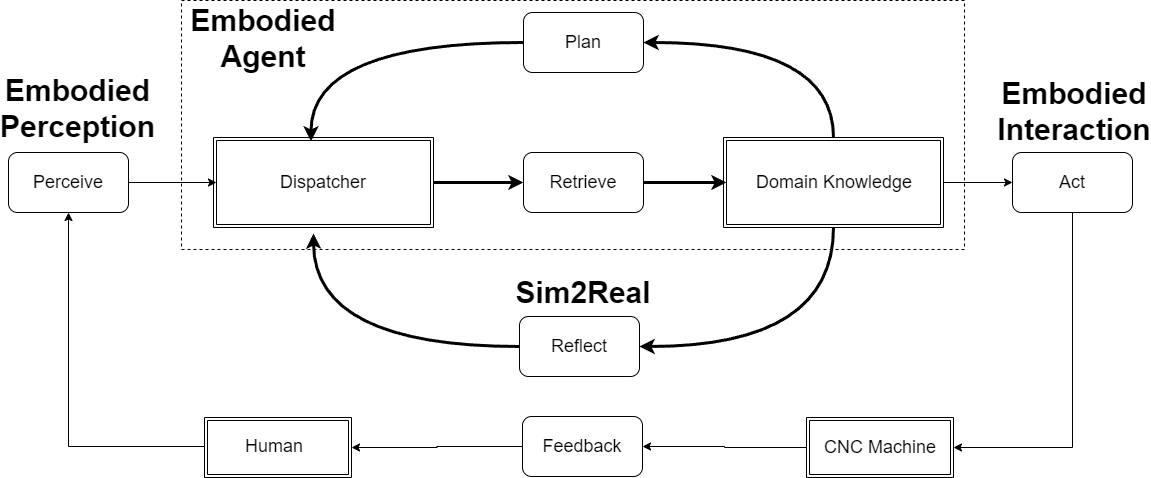
\includegraphics[width=\linewidth]{1.png}
    \caption{Network Topology Diagram}
    \label{fig: 1.png}
\end{figure}

\subsection{功能子组件与模块化构建}

\subsubsection{数控系统的具身智能建模与应用}

在具身智能框架下，智能CNC系统的设计通过集成与反馈机制实现了任务的动态优化和自适应控制。具身智能的建模方式为系统提供了从感知到执行的全流程支持，具身感知、知识图谱、仿真验证和闭环控制共同作用，确保任务执行的准确性与高效性。

\textbf{多层次感知与数据融合：}  
具身感知是数控系统建模的基础。通过多模态传感器，系统能够实时监测CNC设备的状态，采集包括振动、温度、工具磨损等在内的关键数据。这些数据不仅用于监测当前任务的执行情况，还通过与历史数据的对比，帮助系统预测设备的健康状态。具身感知模块将来自不同传感器的数据整合为统一的任务背景信息，通过深度学习模型分析这些数据，并提供对任务的优化建议。通过知识图谱，具身感知模块能够将采集到的数据与任务规划、设备状态等关联起来，从而为任务的后续步骤提供更可靠的依据。例如，在加工过程中，系统会根据设备的实时状态调整切削速度或工具路径，确保任务在执行过程中达到最佳效果。

\textbf{知识图谱驱动的任务优化：}  
知识图谱是具身智能模型的核心组件之一，它不仅用于存储系统中的关键任务信息，还能动态更新并指导任务执行。在建模过程中，知识图谱整合了来自多源信息的加工知识，如技术手册、历史操作数据、加工工艺等。这些信息帮助系统对任务进行优化和调整。通过知识图谱的驱动，系统能够实时调整任务规划。例如，系统可以根据当前加工环境中的实际情况选择最佳的工具和加工路径，从而减少加工时间并提高效率。知识图谱通过对任务背景的全面了解和动态更新，支持了任务的优化执行，使得数控系统能够在面对复杂任务时表现出较强的适应性和智能化水平。

\textbf{基于仿真的任务验证与调整：}  
在具身智能模型中，Sim2Real模块通过虚拟仿真确保任务执行的可行性。Sim2Real不仅用于任务执行前的初步验证，还在仿真过程中对任务进行动态调整。通过对任务环境的虚拟化，Sim2Real模块能够提前发现任务执行中的潜在问题。仿真不仅包括几何结构的模拟，还结合了物理属性和设备状态的仿真。通过这种方式，系统能够确保虚拟环境与真实任务执行环境的高度一致性，从而减少任务执行中的错误和效率损失。在实际执行过程中，系统还会根据仿真反馈不断优化G代码，确保实际执行与仿真中的预期结果一致。

\textbf{决策代理与反馈闭环控制：}  
具身代理的建模方式强调了任务的自适应性和闭环控制。在具身智能系统中，具身代理模块不仅负责任务的分解与执行，还利用强化学习和深度学习技术对任务执行进行自我调整。每次任务执行都会产生新的数据，帮助代理模块不断优化未来的任务规划和决策。具身代理通过实时监控任务执行情况，分析反馈信息，并根据这些数据做出调整。例如，如果任务执行过程中某个加工步骤的精度不够，代理模块可以重新生成G代码并调整加工参数，以提高任务的完成度和精度。通过这种自适应的学习机制，具身代理确保了数控系统在面对复杂任务时的高效和准确。

在数控系统的具身智能建模中，感知、知识图谱、仿真和决策代理相互协作，通过多层次的数据融合和反馈机制，确保任务执行的高效性和精准性。具身智能的建模方式不仅提升了系统的自动化水平，还增强了系统在复杂制造任务中的适应性和自我优化能力。通过仿真和反馈的闭环控制，系统能够在任务执行前进行优化，并在任务执行过程中根据反馈数据进行动态调整，实现智能化的CNC加工流程。

\begin{figure}[hbt]
    \centering
    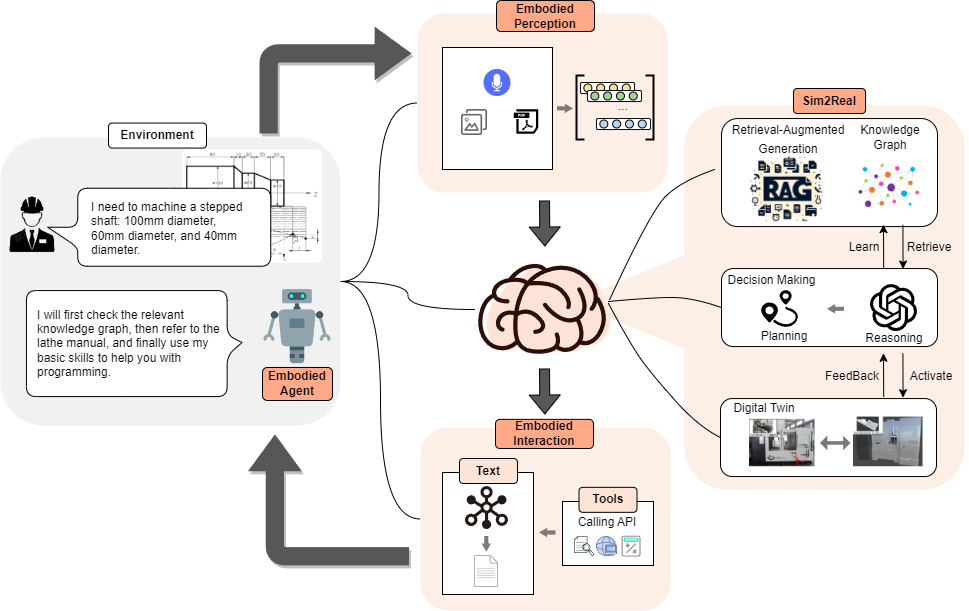
\includegraphics[width=\linewidth]{2.png}
    \caption{Network Topology Diagram}
    \label{fig: 2.png}
\end{figure}

\subsubsection{具身感知模块}

具身感知模块是智能CNC系统的重要组成部分，负责通过多模态传感器网络实时监测设备的状态，并将这些数据用于任务规划和实时调整。该模块通过振动、温度、工具磨损等传感器采集设备运行的物理状态信息，并将这些数据融合处理，与历史数据和知识图谱进行对比分析。这一过程不仅帮助系统识别设备运行中的异常情况，还为任务规划提供数据支持。在任务执行过程中，具身感知模块不断提供实时反馈，支持系统对任务进行动态调整，如调整切削路径、修改加工参数等，以优化加工精度和任务执行效率。通过与任务规划模块的协作，具身感知模块确保了CNC系统能够灵活适应复杂的加工环境，同时通过闭环反馈实现自适应控制，提升了任务执行的安全性和可靠性。

\begin{figure}[hbt]
    \centering
    \includegraphics[width=\linewidth]{3.png}
    \caption{Network Topology Diagram}
    \label{fig: 3.png}
\end{figure}

\subsubsection{具身交互模块}

具身交互模块是智能CNC系统的核心组成部分，负责解析用户指令并动态调整加工任务执行策略。该模块基于自然语言处理（NLP）技术，能够理解操作员的输入，并将其转化为具体的加工步骤，同时结合知识图谱与历史数据进行优化。系统在交互过程中，通过多轮对话管理机制不断完善加工参数，并在必要时引导用户补充关键信息。这一过程不仅提升了任务执行的准确性，还增强了CNC系统对复杂加工需求的适应能力。在任务执行过程中，具身交互模块通过实时反馈机制调整G代码生成策略，优化加工路径、调整进给速度等参数，以确保加工精度和生产效率。通过与具身感知模块及任务规划模块的协同作用，具身交互模块使CNC系统能够更高效地响应操作员需求，提升整体智能化水平，并实现对加工过程的实时优化和精准控制。

\begin{figure}[hbt]
    \centering
    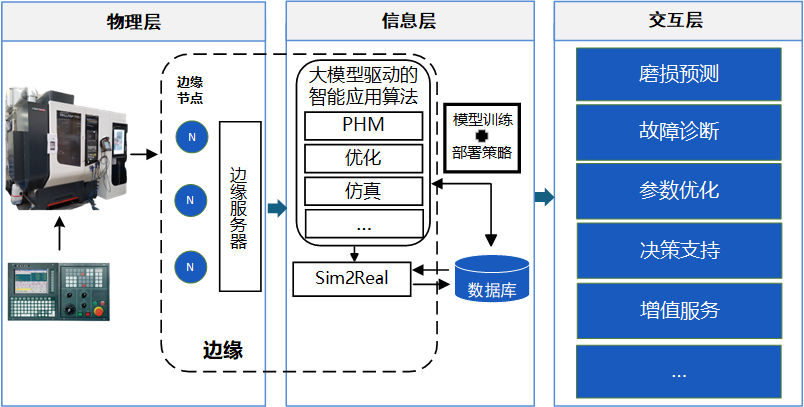
\includegraphics[width=\linewidth]{4.png}
    \caption{Network Topology Diagram}
    \label{fig: 4.png}
\end{figure}

\subsubsection{Sim2Real模块}

Sim2Real模块是智能CNC系统中的关键组件，负责在任务执行前对加工过程进行虚拟仿真，并在执行过程中进行动态优化。该模块利用数值模拟技术对加工任务进行预演，验证G代码的可行性，并识别潜在的加工风险，如刀具干涉、过切或路径优化问题。通过结合知识图谱和历史加工数据，Sim2Real模块能够调整切削参数、优化刀具路径，并在仿真阶段修正不合理的加工策略。在实际加工过程中，该模块持续监测任务执行情况，并将反馈数据与仿真结果进行对比，动态调整G代码以确保加工精度和稳定性。通过与具身感知模块和具身交互模块的协同作用，Sim2Real模块提升了CNC系统对复杂工艺的适应能力，有效降低了加工试错成本，同时增强了系统的可靠性和智能化水平。

\begin{figure}[hbt]
    \centering
    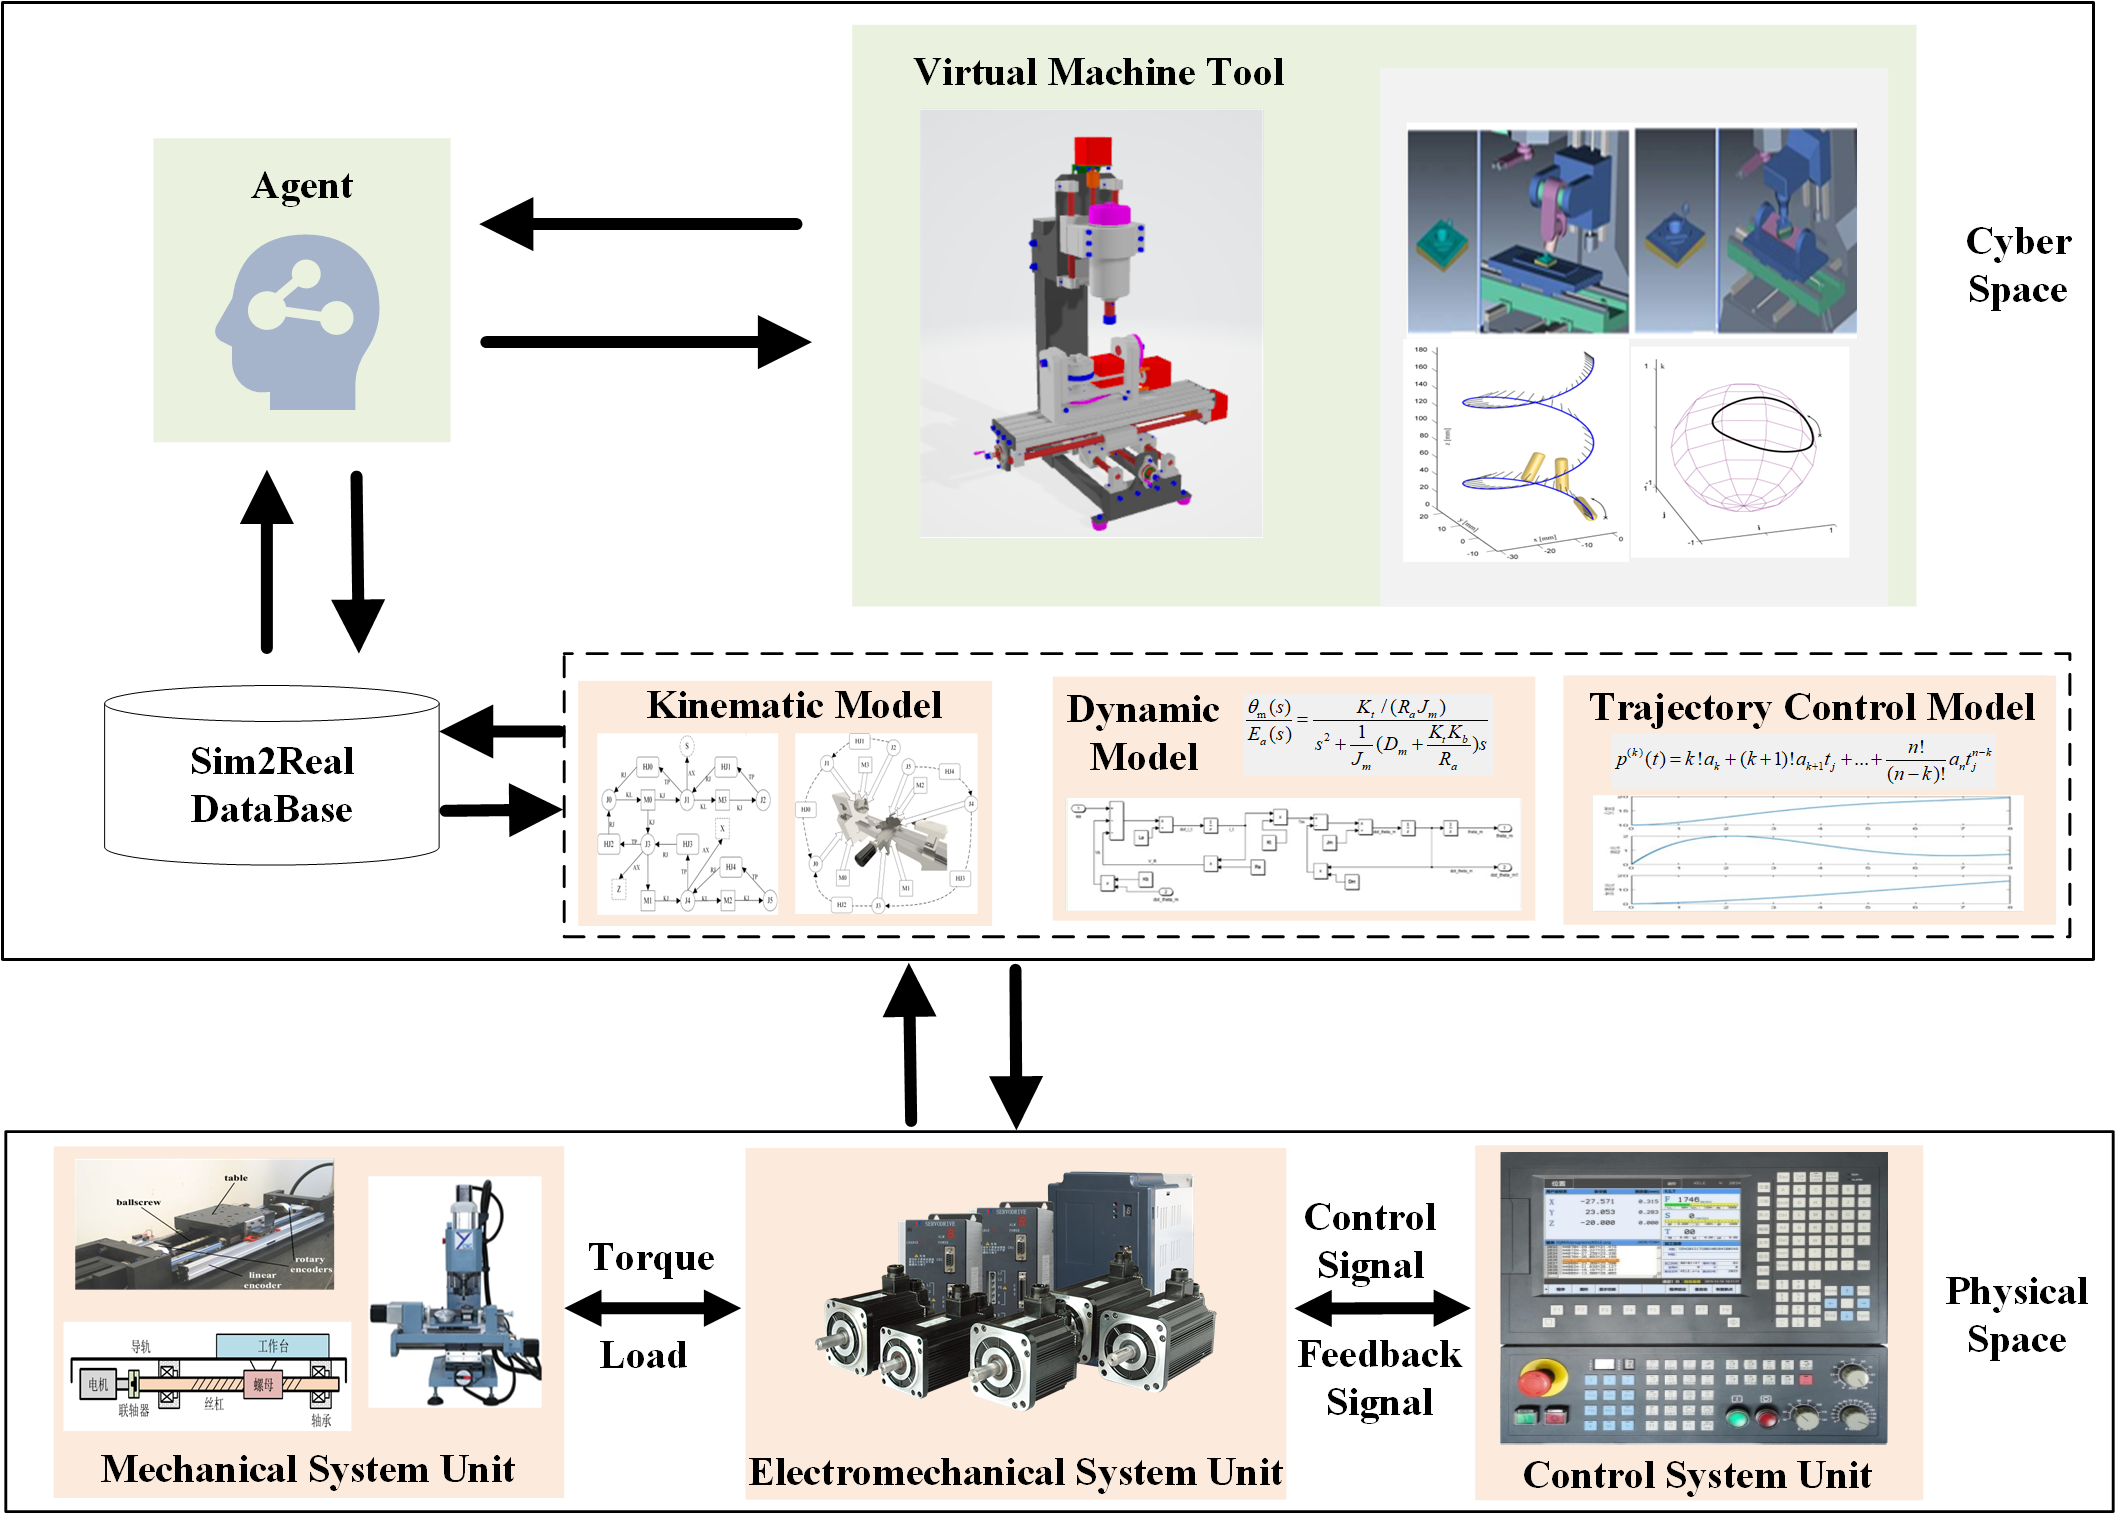
\includegraphics[width=\linewidth]{5.png}
    \caption{Network Topology Diagram}
    \label{fig: 5.png}
\end{figure}

\subsubsection{具身代理模块}

具身代理模块是智能CNC系统的核心决策单元，负责任务的分解、优化与执行。该模块结合大语言模型与知识图谱，对用户输入的加工需求进行深度解析，生成对应的G代码，并动态调整加工策略。具身代理模块通过自适应优化机制，对历史加工数据进行分析，优化刀具路径、调整进给速度，并在执行过程中进行实时调整，以确保加工精度和生产效率。在任务执行过程中，该模块持续接收来自具身感知模块的反馈数据，与Sim2Real模块协同优化加工策略，确保任务的稳定性与可靠性。通过与具身交互模块的配合，具身代理模块能够根据操作员的输入动态调整加工流程，使CNC系统具备更强的智能化和自主优化能力，有效提升复杂加工任务的执行效率和精度。

\begin{figure}[hbt]
    \centering
    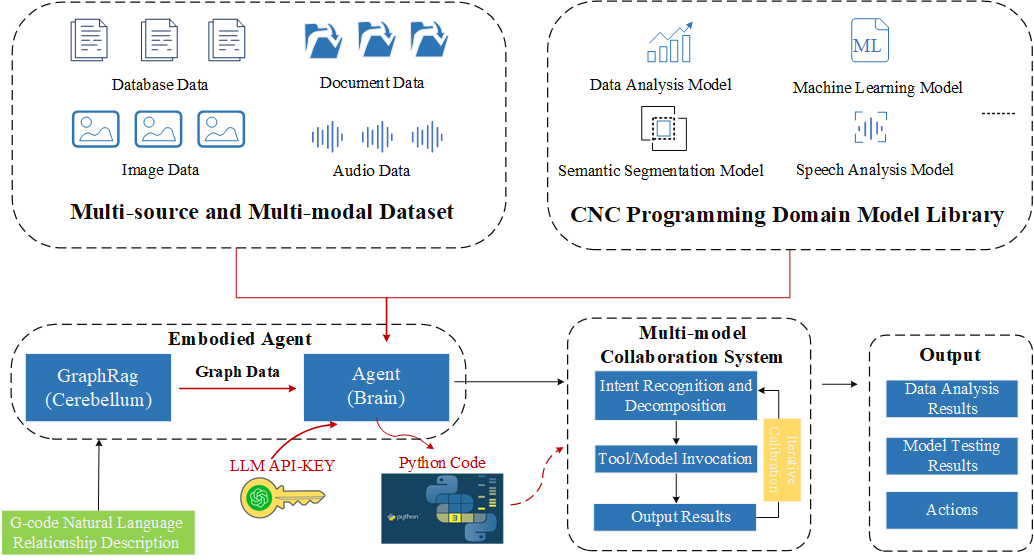
\includegraphics[width=\linewidth]{6.png}
    \caption{Network Topology Diagram}
    \label{fig: 6.png}
\end{figure}

\section{基于具身智能的 G 代码生成模块化方法}

\subsection{系统工作流程概述}

本系统面向自然语言驱动的智能数控（CNC）编程任务，提出了一种基于具身智能理念的 G 代码自动生成方法。整体架构由四个核心模块构成：任务感知与意图识别模块、人机交互与参数补全模块、知识图谱驱动的模板G代码生成模块以及仿真验证与可视反馈模块，各模块之间通过结构化信息流实现高效协同，形成一套面向制造任务全流程的智能编程闭环。

系统的工作流程如图~\ref{fig:system-flow} 所示。用户以自然语言输入形式提出加工任务，例如“我要铣一个深度5毫米的矩形槽，起点在X10Y10”。系统首先通过任务感知模块完成对用户意图的识别与任务分类，提取核心任务类型（如“铣槽”）及关键词标签，并生成初步的语义结构表示。随后，交互模块对任务中参数槽位进行扫描，识别已知与缺失参数，通过主动问答或默认推理方式完成加工要素的补全，确保结构化信息的完整性与准确性。

在获取完整参数后，系统进入模板生成模块流程，利用任务标签和关键词在事先构建的知识图谱中检索适配的 G 代码模板节点。模板节点由经验丰富的操作人员整理而成，具备规范性强、覆盖面广的工程优势。系统依据语义相似度、参数覆盖度与调用频率对候选模板进行排序，选择最佳匹配节点并完成参数注入与语法渲染，输出结构完整、符合工业控制器要求的 G 代码程序。

为验证生成结果的有效性与可用性，系统将最终生成的 G 代码输入至构建于 Unity 平台的虚拟仿真模块中，驱动模型完成路径运动与加工流程模拟。该模块不仅可用于动态呈现加工行为，还能反馈指令执行异常、路径干涉等潜在问题，为程序修正与参数调优提供依据，构建出“自然语言输入—仿真反馈验证”闭环路径。

整套系统架构实现了从“非结构化语言输入”到“结构化可执行程序”之间的自动转译与验证任务。各模块职责明确、边界清晰，既体现了大语言模型在语义理解与交互生成中的能力，也兼顾了知识图谱与规则引擎在工业落地场景中的可控性与稳定性。系统具备良好的扩展性与泛化能力，能够支撑多类型标准加工场景，推动自然语言驱动智能制造的可实现路径。

\begin{figure}[htbp]
    \centering
    \includegraphics[width=0.95\textwidth]{figs/system_flowchart.pdf}
    \caption{自然语言驱动的G代码生成系统整体工作流程}
    \label{fig:system-flow}
\end{figure}

\subsection{面向任务的意图识别算法}

\subsection{交互式参数补全策略}

\subsection{基于知识图谱推理的模板G代码构建}

\subsubsection{模块概述}

本模块作为智能CNC编程系统的核心功能单元，根据用户输入的任务类型与参数信息，从知识图谱中定位适配的G代码模板节点，生成结构完整且具备可执行性的G代码程序。模板内容由经验丰富的操作人员整理，结合典型工艺逻辑抽象生成，具备良好的规范性和适应性。系统通过图谱检索完成模板的精确匹配，并在此基础上进行参数填充与语法规范校验，确保最终输出满足加工控制器的运行要求。
 
模板匹配环节依据任务标签与语义关键词检索图谱节点，通过参数覆盖度与调用历史等因素进行排序筛选。匹配完成后，系统将已知参数注入模板中的预设插槽，对缺失部分进行默认推理或提示补充。G代码拼接后进入语法与执行逻辑验证阶段，包括指令合法性、加工顺序合理性与控制器兼容性等规则判断。模块整体运行稳定，生成结果可控，适用于多类标准加工场景，也为后续仿真验证模块提供了有效输入支撑。

模块在系统中承担从语义输入到程序输出的关键转换任务，与任务识别模块、交互模块及仿真模块形成完整的协同关系。任务识别结果决定模板选择方向，参数交互模块提供填充所需信息，而仿真模块则以本模块输出为基础执行可视化模拟与反馈验证。各模块之间形成清晰的信息流，支撑自然语言驱动的CNC任务执行链路，构建出结构合理、分工明确的智能编程引擎。

\subsubsection{模板节点匹配机制}

模板节点匹配是本模块中关键的起始环节，目标是根据任务识别结果，从知识图谱中选择与当前加工任务最匹配的G代码模板节点。系统构建了结构化的任务模板图谱，每个模板节点包含对应任务类型的通用代码结构、必需参数说明、关键词标签以及适用范围等多种属性信息，用于支持高精度的语义关联与选择。

用户输入的自然语言在完成意图识别与任务解析后，系统将对其与知识图谱的结构适配性进行判断。若当前任务类型能够与图谱中的模板节点建立有效关联，且语义表达具备足够的匹配度，则进入模板匹配流程；对于无法建立图谱关联的输入，系统将切换至其他处理路径，包括基于大语言模型的交互式补全与辅助生成机制。该判断机制提升了系统的容错能力，避免模板系统误处理非结构化表达，确保模块调用的精准性与任务处理的稳定性。

模板匹配过程中，系统首先根据任务标签在图谱中检索候选模板节点集合。关键词扩展策略用于提升召回范围，结合任务名称、工艺短语、常用表达等，构建多维语义匹配集。模板节点构建阶段已预设多语言词汇与拼音别名索引，提升了系统对多样化语言输入的适应性。

在候选节点集合中，系统通过综合评分机制对各模板进行排序。评分函数引入关键词语义相似度、参数覆盖度与模板调用频率等维度指标，计算方式如下：

\begin{equation}
    \text{Score} = \alpha \cdot \text{KeywordSim} + \beta \cdot \text{SlotCoverage} + \gamma \cdot \text{UsageFrequency}
\end{equation}

其中，KeywordSim 衡量任务关键词与模板关键词之间的语义接近程度，SlotCoverage 表示用户输入参数与模板所需参数之间的覆盖比例，UsageFrequency 反映该模板在历史任务调用中的频率或推荐优先级。该策略在提升模板命中率的同时，有效兼顾了语义一致性与结构适用性。

得分最高的模板节点将被选作当前任务的G代码结构基准，并进入参数注入与代码渲染流程。该匹配机制在大量实际任务中表现出良好的稳定性与适应性，能够准确响应多样化自然语言输入，在保证程序结构规范性的同时提升了系统整体的处理效率与智能水平。

\subsubsection{参数注入与规则驱动渲染}

完成模板节点匹配后，系统将任务参数注入G代码模板结构中的各个预设插槽，并根据工业控制逻辑完成模板渲染，生成符合语法规范的完整G代码程序。模板以结构化方式组织，包含若干由占位符标识的插槽字段，用于承载用户输入或系统推理得到的加工参数。模板样例如下所示：

\begin{verbatim}
G00 X{{start\_x}} Y{{start\_y}}
G01 Z{{depth}} F{{feed\_rate}}
\end{verbatim}

模板填充过程以参数完整性与语义一致性为核心原则，主要包括以下几个阶段。首先，系统对用户输入进行参数匹配，将具名参数值与模板插槽进行一一对应，并对单位格式进行标准化处理，确保数值表达的统一性。若存在部分参数缺失，系统将根据任务类型引入默认值补全策略，或触发交互模块请求用户补充输入，以提升参数完整度。

在参数值注入完成后，系统执行类型与范围校验，过滤非法值和潜在冲突配置。例如，当加工材料为铝合金时，系统将对进给速度与主轴转速设定更高的推荐区间，并在必要时进行约束修正。对于结构性组合字段，如刀具路径、起点位置等，系统还引入上下文推理机制，将单个参数转换为复合字段，实现更高层级的指令拼装能力。

渲染完成的G代码在结构上具有良好的工程规范性，指令段清晰、参数明确、语法合法，可直接用于后续仿真验证与实际设备控制。相比基于语言模型的直接生成方式，该规则驱动的模板填充策略具备更强的可控性与透明性，易于在工业场景中快速部署与调试，适应复杂任务的工程要求。

\subsection{仿真驱动验证机制}

\section{Acknowledgments}

The research presented in this paper is part of the subproject titled "Research on the Application Technology of Domestic Five-Axis CNC Systems," with the project number TC220H05S-003, carried out by Shenyang CASNC Technology Co., Ltd. Any opinions, findings, conclusions, or recommendations expressed in this material are those of the authors and do not necessarily reflect the official views of Shenyang CASNC Technology Co., Ltd.

%% The Appendices part is started with the command \appendix;
%% appendix sections are then done as normal sections
%% \appendix

%% \section{}
%% \label{}

%% If you have bibdatabase file and want bibtex to generate the
%% bibitems, please use
%%

\bibliographystyle{elsarticle-num} 
\bibliography{ref}

%% else use the following coding to input the bibitems directly in the
%% TeX file.

% \begin{thebibliography}{00}

% %% \bibitem{label}
% %% Text of bibliographic item

% \bibitem{}

% \end{thebibliography}
\end{document}
\endinput
%%
%% End of file `elsarticle-template-num.tex'.
